\section{Preliminary Findings}
 
To develop a conceptual framework for improving tool recommendations, we first examined existing methods for making tool recommendations.

\subsection{[\peer] ``How Software Users Recommend Tools to Each Other" (Completed, Spring 2017)}

\subsubsection{Motivation:}

% \subsection{Peer Interactions}

% What are peer interactions?
Software engineering researchers and toolsmiths have created many different development tools to help programmers save time and effort in completing development tasks. These tools provide a variety of useful functionality, however software developers often have limited knowledge of these tools and rarely use them in their work. While many automated system-to-user recommendation systems have been developed to increase awareness and adoption of development tools, prior work shows that user-to-user tool recommendations, or \textit{peer interactions}, are the most effective method for discovering new tools. There is limited research examining why user-to-user recommendations are so effective, and to better understand why users prefer recommendations from peers we conducted a user study to observe peer interactions and analyze different characteristics of the recommendations. The characteristics we analyzed were motivated by psychology and persuasion theory as well as prior research examining peer interactions, and provide insights into why tool recommendations between peers is effective and implications for improving automated recommender systems.

\subsubsection{Peer Interactions:}

\textit{Peer interactions} are defined as the process of discovering tools from colleagues during normal work activities~\cite{Murphy-Hill2011PeerInteraction}. Murphy-Hill and colleagues examined seven modes of tool discovery in software engineering, including peer interactions, random tool encounters, tutorials, discussion threads, written descriptions, and social media. They discovered that peer interactions were the most effective way developers learn about new tools~\cite{Murphy-Hill2015HowDoUsers,Murphy-Hill2011PeerInteraction}. There are two types of peer interactions that differ on how the recommendation is made between two colleagues: \textit{peer observation} refers to when a user sees a colleague using an unfamiliar tool that they are unaware of and \textit{peer recommendation} is when a user sees a colleague completing a task inefficiently and suggests a tool. To recognize peer interactions, we developed a model based of of the GOMS (Goals, Operators, Methods, and Selection rules) model in Human-Computer Interaction~\cite{diaper2003handbook}. This model for recognizing peer interactions, shown in Figure~\ref{fig:rec-model}, is defined for two colleagues working together in a pair programming scenario where the user actively operating the keyboard and mouse is the driver and their peer is the navigator~\cite{WilliamsPairProgramming}. In Task Analysis, both peers analyze the task and develop a strategy to complete it. Task Execution refers to when the driver begins executing their strategy and the navigator notices a mismatch. Finally, in the Dialogue a tool is recommended by the navigator inquiring about the driver's tool or suggesting a new tool to complete the task more efficiently.

\noindent
\begin{figure}
\centering
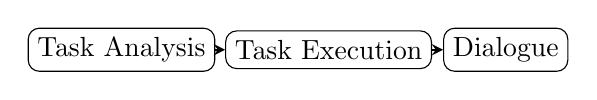
\begin{tikzpicture}
\node (task) [rectangle, rounded corners,text centered, draw=black,node distance=2.5cm] {Task Analysis};
\node (exec) [rectangle, rounded corners,text centered, draw=black, right of=task, node distance=2.63cm] {Task Execution};
\node (dial) [rectangle, rounded corners,text centered, draw=black, right of=exec,node distance=2.25cm] {Dialogue};
\tikzstyle{arrow} = [thick,->,>=stealth]
\draw [arrow] (task) -- (exec);
\draw [arrow] (exec) -- (dial);
\end{tikzpicture}
\caption{Recommendation Model}
\label{fig:rec-model}
\end{figure}

\subsubsection{Research Question:}

\begin{itemize}
  \item[\textbf{RQ}] What characteristics of peer interactions make recommendations effective?
\end{itemize}

\subsubsection{Methodology:}

To evaluate peer interactions in this study, we designed a mixed-methods approach to collect qualitative and quantitative data collected from observing participants.

\paragraph{Participants.} To evaluate the effectiveness of peer interactions, we observed pairs of software users completing data analysis tasks. We recruited undergraduate and graduate students at North Carolina State University as well as professional analysts from the NC State Laboratory for Analytic Sciences\footnote{https://ncsu-las.org/} (LAS) to participate in our study. We observed 13 pairs of participants in total, seven student pairs and six LAS pairs. We requested participants complete a questionnaire survey to collect demographic information and conducted a semi-structured post-interview to gather more data for our results. 

\paragraph{Tasks.} The study tasks involved analyzing data from the Titanic shipwreck and solving problems based on the Kaggle data science competition~\cite{KaggleTitanic}. For our study we did not examine for correctness in task completion, but were interested in how participants recommended tools to each other to solve the tasks. We allowed participants to use the software of their choice for the tasks, but prohibited Internet use to prevent participants form looking up information about the tasks or how to use tools during the study. More information on the tasks, datasets, and study materials are publicly available online.\footnote{http://www4.ncsu.edu/~dcbrow10/files/peer-interaction/study.html} For each session, we screen and voice recorded the participants while they completed the tasks.

\paragraph{Characteristics.} We explored five characteristics of peer interactions to determine what makes them effective: Politeness, Persuasiveness, Receptiveness, Time Pressure, and Tool Observability. These characteristics were motivated from research in psychology and qualitative results from Murphy-Hill's prior work on peer interactions~\cite{Murphy-Hill2015HowDoUsers}. We used psychology research to compile a list of criteria for politeness~\cite{LeechPolite}, persuasiveness~\cite{ShenPersuasive}, and receptiveness~\cite{Fogg2009Persuasive}. We searched for statements made by participants about the time and pace of the session to observe time pressure. Tool observability refers to whether or not a tool is visible through a user interface. 
 
\paragraph{Data Analysis.} To measure effectiveness, each software tool recommendation between participants was categorized as \textit{effective}, \textit{ineffective}, and \textit{unknown}. For effective recommendations, the recommendee used a tool after it was suggested by their partner for the remainder of their session for a majority of the opportunities it was applicable. For ineffective recommendations, the recommendee mostly ignored a tool recommended by their partner when they had a chance to utilize it in the study. Finally, unknown recommendations were the case where there was not another opportunity for the recommendee to use a suggested tool for the rest of their study session.

Two researchers independently viewed recordings of each session to note instances of tool recommendations and categorize the peer interactions based on the criteria defined for each of these characteristics, before coming together to discuss. We calculated our inter-rater agreement using Cohen's Kappa for politeness ($\kappa$ = 0.50), persuasiveness ($\kappa$ = 0.28), and 
receptiveness ($\kappa$ = 0.51).

\subsubsection{Results:}

These results were published in the 2017 Visual Languages and Human-Centric Computing (VL/HCC) conference~\cite{VLHCC}. In total we discovered 142 total recommendations between participants in out study: 71 effective; 35 ineffective; and 36 unknown. Out of the five peer interaction characteristics we analyzed, \textit{receptiveness} was the only characteristic that significantly impacted the outcome of a tool recommendation between peers (Wilcoxon, \textit{p} = 0.0002). Our results show that tool recommendations targeting the receptivity of users when making suggestions are more effective than those that don't. In this study, we defined receptiveness based on prior work by Fogg on designing persuasive technology~\cite{Fogg2009Persuasive}. There were two criteria for observing receptiveness: \textit{\textbf{Demonstrate Desire}} and \textit{\textbf{Familiarity}}. In future work, we plan to design and evaluate automated recommendation approaches that prioritize receptiveness to make more effective suggestions to developers.

\subsection{[\sorry] ``Sorry to Bother You: Designing Bots for
Effective Recommendations" (Completed, Spring 2019)}

\subsubsection{Motivation:}

While recommendations between humans are the most effective, they are not always be the most practical way to increase awareness of useful development tools. For example, even though Murphy-Hill and colleagues discovered that developers prefer peer interactions for tool discovery, they also found that peer interactions occur less frequently in the workplace~\cite{Murphy-Hill2011PeerInteraction}. As development teams become larger and more distributed, effective automated recommendations are necessary to improve tool adoption among software engineers.

Bots are useful for automating tasks and improving user effectiveness and efficiency~\cite{StoreyBots}. However, they can also be inconvenient during interactions with humans. To better understand the impact of bots on human behavior and identify a baseline for automated recommendations, we evaluated making development tool recommendations to software engineers using our \tele. In this study, we gathered feedback from developers receiving recommendations from a naive version of \tool to better understand user reactions to automated recommendations and to set the groundwork for designing better solutions for future approaches to improve the effectiveness of automated suggestions from bots.

\subsubsection{\tele:}

To evaluate a basic design for making automated recommendations, we developed \tele. This approach behaves similar to a telemarketer in that it ``calls" users to deliver a static message that never deviates from the script and lacks the social context necessary to adjust messages and respond to questions. \tele sends developers a generic message with information about the tool, displays a generic code snippet with a common programming error, and provides sample output from the tool. This is not the best approach for making recommendations, however we implemented this simple design to better understand how bots influence human behavior and how developers respond to automated recommendations. With this naive design, we identified a baseline to motivate integrating concepts from nudge theory into future automated recommendation designs. 

\subsubsection{Methodology:}

\paragraph{Implementation.} To evaluate our \tele approach, we implemented \tool to make basic tool recommendations to GitHub developers. \tool integrates this simple approach by making generic recommendations as automated pull requests on repositories. On GitHub, pull requests are the preferred method to propose changes to repositories\footnote{https://help.github.com/articles/about-pull-requests/}. Automated pull requests have also been used by bots in related work, for example by Mirhosseini and colleagues to encourage GitHub developers to upgrade out-of-date dependencies for repositories~\cite{SamUgrade}. Figure~\ref{fig:tele} presents a screenshot of a recommendation from our system for this study. In this experiment, \tool recommendations provided basic information about the Java static analysis tool \EP  (Fig.~\ref{fig:tele}.A). It also presents a simple coding error in Java, using ``\texttt{==}" to evaluate string equality instead of the \texttt{String.equals()} method (Fig.~\ref{fig:tele}.B1), and the corresponding output from \EP reporting a \texttt{StringEquality} error\footnote{http://errorprone.info/bugpattern/StringEquality} (Fig.~\ref{fig:tele}.B2). To make recommendations, \tool automatically adds the \EP plugin to Maven\footnote{http://maven.apache.org}, to Project Object Model (\textit{pom.xml}) configuration files and created automated pull requests with the changes. An example pull request from our system using the \tele can be found here.\footnote{https://github.com/CSC-326/JSPDemo/pull/2}

\begin{figure}
\centering
	\includegraphics[width=0.5\textwidth]{images/pull.png}
	\caption{Example \tele recommendation}	
	\label{fig:tele} 
\end{figure}

\paragraph{Projects.}

We sampled public open source software repositories on GitHub used in the evaluation for Repairnator\footnote{https://github.com/Spirals-Team/repairnator/blob/master/resources/data/results-buildtool.csv}~\cite{Repairnator}, an automated program repair bot~\cite{Repairnator}. Our evaluation sought to determine the effectiveness of our \tele recommendation approach to developers working on real-world software applications. The projects we selected projects were required to be primarily written in Java 8 or higher, successfully validate and compile with Maven, and not already include \EP in the build configuration. Based on these criteria, we identified 52 projects for our experiment that received an automated pull request recommendation from \tool. The list of projects for this evaluation is available online\footnote{https://go.ncsu.edu/botse-projects}.

\paragraph{Data Analysis.}

To observe the effectiveness of \tele, we categorized automated recommendations as \textit{effective} or \textit{ineffective} based on the status of pull requests. A merged automated pull request from \tool indicates an effective recommendation because the developer showed a willingness to try \EP and integrate the static analysis tool  into the build for their repository by merging our changes into their code base. A closed or ignored pull request left open from our system indicates an ineffective recommendation because the developers did not attempt to integrate the tool into their projects. We observed the automated pull requests for one week to categorize the recommendations. The rate of effectiveness was calculated by measuring the percentage of merged pull requests out of the total sent.

Additionally, we encouraged developers to provide feedback on pull requests by asking them to ``Please feel free to add any comments below explaining why you did or did not find this recommendation useful". This was done to gather qualitative data on how developers reacted to receiving \tele recommendations from \tool. We aggregated and analyzed the comments made by GitHub developers on our automated recommendations. Figure~\ref{fig:botse} presents a screenshot of example automated pull requests used in the evaluation for this study.

\begin{figure*}[]
\centering
\subfloat[Pull request recommendation text]{\includegraphics[width=0.5\linewidth]{images/botse1.png}}
\subfloat[Pull request diff updating a \pom file]{\includegraphics[width=0.5\linewidth]{images/botse2.png}}
\caption{Example automated pull request from the \sorry study}
\label{fig:botse}
\end{figure*}

\subsubsection{Results:} 

We found that bots with basic approaches are not effective for influencing human behavior. In our evaluation, \tele only made two successful recommendations out of 52 (4\%). We also observed 10 closed pull requests and 40 recommendations with no response from developers. We received 18 comment responses from developers, most of which were negative feedback. Five of the comments were related to improper formatting of the \textit{pom.xml} file when adding the \EP plugin, and eight were related to our automated pull requests breaking builds for projects. Based on this feedback, we discovered the main drawbacks to the \tele were a lack of \textit{\textbf{social context}} and interfering with \textit{\textbf{developer workflow}}. To provide implications for future automated recommender systems, we propose using concepts from nudge theory improve social context and developer workflow for automated suggestions to software developers. The results of this research have been accepted for publication at the 1st International Workshop on Bots in Software Engineering\footnote{https://botse.github.io/} at ICSE 2019~\cite{BotSE}.

